\subsubsection{Blocking}
\label{sec:optim:block}

\todonaps{THIS}

Since it is likely that geometrically closer points also follow a similar traversal, which is the basis for the Spatial Sort optimization, it is also likely that those points can be processed in blocks, rather than one at a time, thus taking advantage of locality, and preventing the traversal from being evicted too soon from cache.

Instead of traversing the structure for a single point, and iteratively switching points, the new strategy takes advantage of the premisse that Spatial Sort rearranges points so that a small subset of points is likely to be geometrically close to each other. This subset is grouped into a block, and the tree is traversed for that block at the same time.

The root node of the structure is processed for all points of the block. If necessary (depending on the algorithm), if the paths of each point in the block diverge at a given node, it may be necessary to split the block into smaller blocks, each one going to a different node. Given the geometrical proximity, this is only more likely to occur at the last levels of the structure, allowing for some locality to still be gained in the previous levels.

\Cref{fig:sort} illustrates the execution order of a point blocked implementation, compared to the non blocked, sorted implementation.

\begin{figure}[!htp]
	\centering
	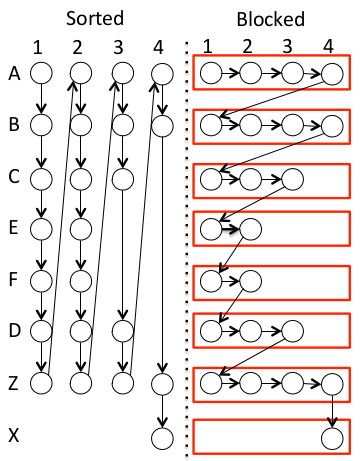
\includegraphics[width=0.6\columnwidth]{pointblocking_blocks}
	\caption{Point Blocking transformation}
	\label{fig:sort}
\end{figure}

It is intuitive to notice that this strategy is only good if the points within a block are likely to follow a similar traversal path, otherwise too much divergence will hinder performance much like the original strategy.